
% this file is called up by thesis.tex
% content in this file will be fed into the main document

%: ----------------------- introduction file header -----------------------


\begin{savequote}[50mm]
Success is the sum of small efforts, repeated day-in and day-out.
\qauthor{Robert Collier}
\end{savequote}

\chapter{Introduction}
\label{cha:1_Introduction}

% the code below specifies where the figures are stored
\ifpdf
    \graphicspath{{1_introduction/figures/PNG/}{1_introduction/figures/PDF/}{1_introduction/figures/}}
\else
    \graphicspath{{1_introduction/figures/EPS/}{1_introduction/figures/}}
\fi


%-------------------------------------------------------------------------
%Chapter 1 contents:
%- Motivation of the research field: Context-aware systems -> LBS -> GNSS limitation -> Positioning techniques -> DR -> inertial PDR -> inertial PDR + wearables
%- Problem identification: smartphone not a wearable -> potentiality of wrist-worn wearables -> Problem: no wrist-worn PDRS
%- Goal of the thesis: tackle the problem -> how? Splitting it into sub-problems
%- Structure of the thesis
%-------------------------------------------------------------------------

Machine learning (ML) allows developing effective data-driven solutions that allow making smart decisions. The rapid growth of data volumes and sources has increased the efficiency of data-based solutions, making this area more and more important. A closely related field to ML is data mining (DM), \textit{¨to do with the discovery of useful, valid, unexpected, and understandable knowledge from data¨} \cite{torgo2016}. However, with the plethora of statistical learning methods, the explored pattern is usually different and hence, the final decision could be affected \cite{hand2014}. A promising data-driven solution has been recognized via combining or weighting several data analytical methods \cite{breiman1996,breiman2001,freund1997}. This is accepted and promoted by computational intelligence community with the name of ensemble systems \cite{polikar2012,dietterich2002,opitz1999,sagi2018,oza2001,krawczyk2017,zhang2012}. Specific ensemble systems for classification tasks are known as Multiple Classifier Systems (MCSs) \cite{polikar2006,rokach2010,kuncheva2014,wozniak2014}, with the concept of designing, implementing, and validating many classifiers to cope with uncertainty, ambiguity, and complex problems.  Classifier ensembles reside at the intersection of engineering, computing, and mathematics \cite{kuncheva2014}. 

MCS is the methodology where many classifiers are generated and their decisions are combined to get more accurate and stable decisions. Regarding that, MCS should be designed efficiently in all of their stages, from data preprocessing to multioutput decision fusion. Many variants exist either to generate or to combine the group of classifiers, while the majority of the articles and the designed algorithms consider the whole dataset to train each individual. This slows the classification system by adding more computations to train several classifiers from complete data. In addition, ambiguity and uncertainty will be increased. Furthermore, the test time will be more consumed by the individual classifiers to get the final decision.     

Therefore, this thesis aims to propose the development of MCS, to design more efficient and effective classifier ensembles, via incorporating the following strategies:
\begin{itemize} [nosep]
    \item Intelligent data sampling via applying instance selection (IS) techniques.
    \item Building a group of heterogeneous classifiers to increase the diversity inside the decision space.
    \item Applying swarm intelligence (SI) as a soft computing technique to combine the classifier's outputs properly.
    \item Analysis of popular and recent ensemble pruning metrics to get thinner/small-size ensembles, with the significant impact to increase the efficiency and the predictive performance.
\end{itemize}

     

In this chapter, the motivation for this research along with the research questions
that naturally arise are discussed in  Section~\ref{sec:1_1_motivation}. After this, the objectives and contributions are presented in Sections \ref{sec:1_2_opportunity} and \ref{sec:1_3_1_goal}, respectively. Next, the
research methodology is summarised in Section \ref{sec:1_3_automl_and_tf}. Finally,
the research context and the outline of this thesis are presented in Sections \ref{ch1:research-context} and
\ref{sec:1_3_2_DissertationStructure}, respectively.





\section{Motivation and Scope}
\label{sec:1_1_motivation}

MCS performs well since classifiers differ in terms of their inductive biases \cite{geman1992}. With the classical approach of focusing on a highly optimized classifier, various challenges are encountered, e.g., in terms of the data size, the number of classes, the dimensionality of the feature space, the overlap between instances, the balance between class categories, and the nonlinear complexity of the true unknown hypotheses \cite{zhou2012}. A promising alternative is to use a group of classifiers. The true unknown hypothesis can be approximated by searching in various regions. This is one of the main supports of the working mechanisms of MCS, as each classifier exploits the search space differently by using different feature subsets, data samples, or learning mechanisms. The general structure of MCS is depicted in Figure \ref{ch1:MCS-topology} following the classical pattern recognition structure. The set of features describing the objects are input to the classifier ensemble, formed by a set of diverse classifiers \cite{wozniak2014}. Then, an appropriate combination rule fuses the individual classifier outputs to provide the system decision. 


\begin{figure}[!ht]
    \centering
    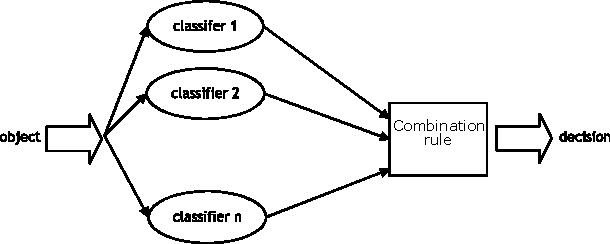
\includegraphics[width=.9\textwidth]{1_introduction/figures/Ch1_MCS-topology.pdf}
    \caption{The canonical topology of MCS, Taken from \cite{wozniak2014}.}
    \label{ch1:MCS-topology}
\end{figure}






A vital phase in building a group of classifiers is to use a suitable fusion strategy to aggregate response decisions \cite{zhou2012,kuncheva2014}. Regarding that, the general accuracy of the ensemble model could be improved by properly tuning the decision weights of individual classifiers. However, the following challenges are encountered in the application of a weight-based combination rule: (1) If the amount of data increases or the number of classifiers becomes large, the search space becomes more complex to determine the proper weight. (2) The search space may be flat or multimodal, namely, there are multiple solutions (weights) that all provide approximately the same accuracy. (3) The assignment of a general weight for each classifier in consideration of its overall accuracy is not efficient for decision fusion because each classifier has different performance capabilities for predicting per-class instances. Answering to that, swarm intelligence (SI)  can be used to identify a pattern or even to tune the weight parameters for multiclassifier decision fusion. In addition, SI handles the multimodal problem by stochastically applying exploration to avoid stagnation at local solutions. 

\textit{In addition}, reducing the training data leads to reducing the in-between classifiers conflict, with the aim to decrease the uncertainty and ambiguity in MCS. However, reducing the training data could affect the learning negatively. Scientific researchers have focused on the selection of the most relevant instances via data preprocessing \cite{garcia2015} to feed the classification model. Regarding that, instance selection (IS) techniques could be applied in advance before training MCS. Hence, the training and the testing times will be further reduced. The combination method should exploit the strengths of individual classifiers' over each class (class-specific weights). For that, SI algorithms can be used to tune the weights of each classifier based on its accuracy to predict a specified class. Furthermore, SI algorithms could compensate the loss in the accuracy of the applied IS techniques.  

A Current subject of interest in MCS is to downsize the ensemble. Downsizing the ensemble (ensemble pruning, ensemble selection, and ensemble forming) is a strategic process by which a subset of ensemble members can be selected while maintaining, even improving, the performance of the original ensemble \cite{mousavi2015}. Ensemble selection can be embedded in the combination method, as in weighted voting where classifiers with lower weights or less than a predefined threshold can be removed \cite{krawczyk2016,li2014}. The ensemble size has an important inconvenience according to the following: \textit{Memory requirements} to store the parameters of all the base learning models, \textit{classification speed} which deteriorates with large ensemble sizes, and the \textit{predictive performance metric} that can be improved by merging a subset of models instead of depending on the whole ensemble members \cite{martinez2009,guo2013,zhou2014}. A possible solution to alleviate those shortcomings can be broadly divided into the following five solutions \cite{onan2017,mendes2012}:
\begin{itemize}[nosep]
    \item Exhaustive search.
    \item Optimization-based search.
    \item Sequential search (greedy methods).
    \item Clustering-based pruning.
    \item Ranking-based pruning (ordering-based pruning).
\end{itemize}

\noindent Regarding that, a promising MCS could be designed to: 
\begin{itemize} [nosep]
    \item Benefit from the downsized data and the downsized classifiers simultaneously.
    \item Form ensemble models quickly, especially when training complex and a large number of individual classifiers.
    \item Improve the size and overall accuracy of the ensemble systems.
    \item Get out more accuracy from the reduced data in comparison with state-of-art ensembles which are trained from non reduced data.
\end{itemize}

Multiple classifier systems are composed of three stages: (A) Forming, (B) Selection, and (C) Aggregation \cite{cruz2018}. The selection process is optional as it is not embedded in many ensemble systems. However, it has been proved that the generalization performance of a subensemble reports superior results over the traditional combination approaches, such as majority voting of the whole ensemble \cite{martinez2009,zhou2002}.
In addition, pruning down the redundant models reduces the memory burden \cite{diao2013}. Furthermore, ensemble selection (ES) is a proven mechanism to enhance the efficiency and elevate the efficacy of classification ensemble systems \cite{cao2018,martinez2009,guo2013, lu2010}.  However, it is not trivial to find the optimal subset of classifiers from a large ensemble as the complexity grows exponentially with the size of the pool. Researchers agreed in common that ES is a combinatorial search problem with $2^{T}-1$ nonempty subsets to be evaluated from pool size, $T$, to find the best subset \cite{tamon2000, tsoumakas2009}. 


Greedy algorithms and heuristic metrics have been proved to be convenient techniques that return near-optimal subsets in fast time. Virtually, an ordered list from the generated classifier pool is formed according to an evaluation function, followed by the selection of models according to this fixed order \cite{cao2018}. Those techniques comprise dissimilar heuristic measures such as: ensemble diversity \cite{lu2010}, ensemble margin \cite{martinez2004,guo2013}, margin hybrid diversity \cite{guo2018}, discriminating classifiers \cite{cao2018}, ensemble error \cite{margineantu1997}, complementary of misclassification \cite{martinez2004}, and relative accuracy with minimum redundancy \cite{cao2018}. In \cite{cavalcanti2016}, since no widely accepted definition to measure the ensemble diversity exists, five pairwise diversity measures are combined to obtain an efficient pruned ensembles. In the literature, those techniques are popular and recognized under the name of ordering-based ensemble pruning with the following merits: 
\begin{itemize} [nosep]
    \item The ordering strategies return subsets that are close to the optimal solution (\textit{Efficacy}) \cite{martinez2009}.
    \item The time complexity of those strategies is low, in comparison with exhaustive or optimization-based search methods (\textit{Efficiency}) \cite{martinez2009}.
    \item Pruning strategies based on base classifier reordering can be easily adjusted to adapt to any given storage and computational restrictions \cite{cao2018,guo2018}.
\end{itemize}


Till now and related to our best knowledge, no recent article has considered the analysis of all those promising metrics together. This research covers that gap by comparing all those new techniques with the best performing techniques found in \cite{martinez2009}, and against other popular baseline metrics. 


Summarising, the following research questions are stated based on the above motivations:


\begin{itemize}[nosep]
\setlength{\itemindent}{-.5in}
   \item $\pmb{Q_1}$. What is the impact of reduced and consistent data on the performance of ensemble learning?
    \item $\pmb{Q_2}$. Is it possible with the search capability of swarm intelligence to enhance the combination of classifiers? 
    \item $\pmb{Q_3}$. What is the effect of combining multiple pruning metrics together?
    \item $\pmb{Q_4}$. What is the effect of downsizing data and downsizing the number of classifiers simultaneously? 
    \item $\pmb{Q_5}$. How the initial classifier pool size and the required subensemble size affect on the performance of heuristic pruning metrics?
    \item $\pmb{Q_6}$. How the heuristic pruning metrics are affected by the individual classifier type?
    \item $\pmb{Q_7}$. How the efficacy of the pruning metrics could be affected by binary and multiclass tasks?
    \item $\pmb{Q_8}$. How the pruning metrics are effective to reduce the performance variance?
    \item $\pmb{Q_9}$. How the efficiency of the heuristic pruning metrics differs in terms of time and space complexities?
\end{itemize}

	






%\newpage
\section{Objectives}
\label{sec:1_2_opportunity}
As it has been aforementioned, the contribution of this thesis is related to the design of MCS. To make an intersection between IS, MCS, and SI, with the aim to increase the efficiency and the efficacy of classifier ensemble systems. Furthermore, to analyze the popular and the recent classifier ensemble pruning metrics. Based on the formulated research questions, the following objectives should be achieved.  


\begin{itemize}
    \item $\textbf{Objective  1}$. To build more diverse and highly accurate MCS, only from a reduced portion of the available data. \textit{This objective corresponds to research questions $Q_1$ and $Q_2$}.  
    \item $\textbf{Objective  2}$. Increasing the efficiency of MCS and going beyond what can be achieved from ensemble pruning methods. \textit{This objective corresponds to research questions $Q_3$ and $Q_4$}.  
    \item $\textbf{Objective  3}$. Grouping and analyzing fast and accurate heuristic metrics for MCS pruning. \textit{This objective corresponds to research questions $Q_5$ to $Q_9$}  
   
\end{itemize}


